%% bare_jrnl.tex
%% V1.4b
%% 2015/08/26
%% by Michael Shell
%% see http://www.michaelshell.org/
%% for current contact information.
%%
%% This is a skeleton file demonstrating the use of IEEEtran.cls
%% (requires IEEEtran.cls version 1.8b or later) with an IEEE
%% journal paper.
%%
%% Support sites:
%% http://www.michaelshell.org/tex/ieeetran/
%% http://www.ctan.org/pkg/ieeetran
%% and
%% http://www.ieee.org/

%%*************************************************************************
%% Legal Notice:
%% This code is offered as-is without any warranty either expressed or
%% implied; without even the implied warranty of MERCHANTABILITY or
%% FITNESS FOR A PARTICULAR PURPOSE! 
%% User assumes all risk.
%% In no event shall the IEEE or any contributor to this code be liable for
%% any damages or losses, including, but not limited to, incidental,
%% consequential, or any other damages, resulting from the use or misuse
%% of any information contained here.
%%
%% All comments are the opinions of their respective authors and are not
%% necessarily endorsed by the IEEE.
%%
%% This work is distributed under the LaTeX Project Public License (LPPL)
%% ( http://www.latex-project.org/ ) version 1.3, and may be freely used,
%% distributed and modified. A copy of the LPPL, version 1.3, is included
%% in the base LaTeX documentation of all distributions of LaTeX released
%% 2003/12/01 or later.
%% Retain all contribution notices and credits.
%% ** Modified files should be clearly indicated as such, including  **
%% ** renaming them and changing author support contact information. **
%%*************************************************************************


% *** Authors should verify (and, if needed, correct) their LaTeX system  ***
% *** with the testflow diagnostic prior to trusting their LaTeX platform ***
% *** with production work. The IEEE's font choices and paper sizes can   ***
% *** trigger bugs that do not appear when using other class files.       ***                          ***
% The testflow support page is at:
% http://www.michaelshell.org/tex/testflow/



\documentclass[journal]{IEEEtran}
%
% If IEEEtran.cls has not been installed into the LaTeX system files,
% manually specify the path to it like:
% \documentclass[journal]{../sty/IEEEtran}


\usepackage{url}
\usepackage{graphicx}
\usepackage{float}
\usepackage{subfig}
\usepackage{algorithm}  
\usepackage{algpseudocode}  
\usepackage{amsmath}  
\renewcommand{\algorithmicrequire}{\textbf{Input:}}  % Use Input in the format of Algorithm  
\renewcommand{\algorithmicensure}{\textbf{Output:}} % Use Output in the format of Algorithm
\newcommand*{\Break}{\textbf{break}}
\usepackage{booktabs}
\usepackage{array}
\usepackage{wrapfig}
\usepackage{amsfonts}
\usepackage{epstopdf}
\usepackage{makecell}
\usepackage{caption}
\newcommand{\subsubsubsection}[1]{\paragraph{#1}\mbox{}\\}
\setcounter{secnumdepth}{4} % how many sectioning levels to assign numbers to
\setcounter{tocdepth}{4} % how many sectioning levels to show in ToC

% Some very useful LaTeX packages include:
% (uncomment the ones you want to load)


% *** MISC UTILITY PACKAGES ***
%
%\usepackage{ifpdf}
% Heiko Oberdiek's ifpdf.sty is very useful if you need conditional
% compilation based on whether the output is pdf or dvi.
% usage:
% \ifpdf
%   % pdf code
% \else
%   % dvi code
% \fi
% The latest version of ifpdf.sty can be obtained from:
% http://www.ctan.org/pkg/ifpdf
% Also, note that IEEEtran.cls V1.7 and later provides a builtin
% \ifCLASSINFOpdf conditional that works the same way.
% When switching from latex to pdflatex and vice-versa, the compiler may
% have to be run twice to clear warning/error messages.






% *** CITATION PACKAGES ***
%
%\usepackage{cite}
% cite.sty was written by Donald Arseneau
% V1.6 and later of IEEEtran pre-defines the format of the cite.sty package
% \cite{} output to follow that of the IEEE. Loading the cite package will
% result in citation numbers being automatically sorted and properly
% "compressed/ranged". e.g., [1], [9], [2], [7], [5], [6] without using
% cite.sty will become [1], [2], [5]--[7], [9] using cite.sty. cite.sty's
% \cite will automatically add leading space, if needed. Use cite.sty's
% noadjust option (cite.sty V3.8 and later) if you want to turn this off
% such as if a citation ever needs to be enclosed in parenthesis.
% cite.sty is already installed on most LaTeX systems. Be sure and use
% version 5.0 (2009-03-20) and later if using hyperref.sty.
% The latest version can be obtained at:
% http://www.ctan.org/pkg/cite
% The documentation is contained in the cite.sty file itself.






% *** GRAPHICS RELATED PACKAGES ***
%
\ifCLASSINFOpdf
% \usepackage[pdftex]{graphicx}
% declare the path(s) where your graphic files are
% \graphicspath{{../pdf/}{../jpeg/}}
% and their extensions so you won't have to specify these with
% every instance of \includegraphics
% \DeclareGraphicsExtensions{.pdf,.jpeg,.png}
\else
% or other class option (dvipsone, dvipdf, if not using dvips). graphicx
% will default to the driver specified in the system graphics.cfg if no
% driver is specified.
% \usepackage[dvips]{graphicx}
% declare the path(s) where your graphic files are
% \graphicspath{{../eps/}}
% and their extensions so you won't have to specify these with
% every instance of \includegraphics
% \DeclareGraphicsExtensions{.eps}
\fi
% graphicx was written by David Carlisle and Sebastian Rahtz. It is
% required if you want graphics, photos, etc. graphicx.sty is already
% installed on most LaTeX systems. The latest version and documentation
% can be obtained at: 
% http://www.ctan.org/pkg/graphicx
% Another good source of documentation is "Using Imported Graphics in
% LaTeX2e" by Keith Reckdahl which can be found at:
% http://www.ctan.org/pkg/epslatex
%
% latex, and pdflatex in dvi mode, support graphics in encapsulated
% postscript (.eps) format. pdflatex in pdf mode supports graphics
% in .pdf, .jpeg, .png and .mps (metapost) formats. Users should ensure
% that all non-photo figures use a vector format (.eps, .pdf, .mps) and
% not a bitmapped formats (.jpeg, .png). The IEEE frowns on bitmapped formats
% which can result in "jaggedy"/blurry rendering of lines and letters as
% well as large increases in file sizes.
%
% You can find documentation about the pdfTeX application at:
% http://www.tug.org/applications/pdftex





% *** MATH PACKAGES ***
%
%\usepackage{amsmath}
% A popular package from the American Mathematical Society that provides
% many useful and powerful commands for dealing with mathematics.
%
% Note that the amsmath package sets \interdisplaylinepenalty to 10000
% thus preventing page breaks from occurring within multiline equations. Use:
%\interdisplaylinepenalty=2500
% after loading amsmath to restore such page breaks as IEEEtran.cls normally
% does. amsmath.sty is already installed on most LaTeX systems. The latest
% version and documentation can be obtained at:
% http://www.ctan.org/pkg/amsmath





% *** SPECIALIZED LIST PACKAGES ***
%
%\usepackage{algorithmic}
% algorithmic.sty was written by Peter Williams and Rogerio Brito.
% This package provides an algorithmic environment fo describing algorithms.
% You can use the algorithmic environment in-text or within a figure
% environment to provide for a floating algorithm. Do NOT use the algorithm
% floating environment provided by algorithm.sty (by the same authors) or
% algorithm2e.sty (by Christophe Fiorio) as the IEEE does not use dedicated
% algorithm float types and packages that provide these will not provide
% correct IEEE style captions. The latest version and documentation of
% algorithmic.sty can be obtained at:
% http://www.ctan.org/pkg/algorithms
% Also of interest may be the (relatively newer and more customizable)
% algorithmicx.sty package by Szasz Janos:
% http://www.ctan.org/pkg/algorithmicx




% *** ALIGNMENT PACKAGES ***
%
%\usepackage{array}
% Frank Mittelbach's and David Carlisle's array.sty patches and improves
% the standard LaTeX2e array and tabular environments to provide better
% appearance and additional user controls. As the default LaTeX2e table
% generation code is lacking to the point of almost being broken with
% respect to the quality of the end results, all users are strongly
% advised to use an enhanced (at the very least that provided by array.sty)
% set of table tools. array.sty is already installed on most systems. The
% latest version and documentation can be obtained at:
% http://www.ctan.org/pkg/array


% IEEEtran contains the IEEEeqnarray family of commands that can be used to
% generate multiline equations as well as matrices, tables, etc., of high
% quality.




% *** SUBFIGURE PACKAGES ***
%\ifCLASSOPTIONcompsoc
%  \usepackage[caption=false,font=normalsize,labelfont=sf,textfont=sf]{subfig}
%\else
%  \usepackage[caption=false,font=footnotesize]{subfig}
%\fi
% subfig.sty, written by Steven Douglas Cochran, is the modern replacement
% for subfigure.sty, the latter of which is no longer maintained and is
% incompatible with some LaTeX packages including fixltx2e. However,
% subfig.sty requires and automatically loads Axel Sommerfeldt's caption.sty
% which will override IEEEtran.cls' handling of captions and this will result
% in non-IEEE style figure/table captions. To prevent this problem, be sure
% and invoke subfig.sty's "caption=false" package option (available since
% subfig.sty version 1.3, 2005/06/28) as this is will preserve IEEEtran.cls
% handling of captions.
% Note that the Computer Society format requires a larger sans serif font
% than the serif footnote size font used in traditional IEEE formatting
% and thus the need to invoke different subfig.sty package options depending
% on whether compsoc mode has been enabled.
%
% The latest version and documentation of subfig.sty can be obtained at:
% http://www.ctan.org/pkg/subfig




% *** FLOAT PACKAGES ***
%
%\usepackage{fixltx2e}
% fixltx2e, the successor to the earlier fix2col.sty, was written by
% Frank Mittelbach and David Carlisle. This package corrects a few problems
% in the LaTeX2e kernel, the most notable of which is that in current
% LaTeX2e releases, the ordering of single and double column floats is not
% guaranteed to be preserved. Thus, an unpatched LaTeX2e can allow a
% single column figure to be placed prior to an earlier double column
% figure.
% Be aware that LaTeX2e kernels dated 2015 and later have fixltx2e.sty's
% corrections already built into the system in which case a warning will
% be issued if an attempt is made to load fixltx2e.sty as it is no longer
% needed.
% The latest version and documentation can be found at:
% http://www.ctan.org/pkg/fixltx2e


%\usepackage{stfloats}
% stfloats.sty was written by Sigitas Tolusis. This package gives LaTeX2e
% the ability to do double column floats at the bottom of the page as well
% as the top. (e.g., "\begin{figure}[!b]" is not normally possible in
	% LaTeX2e). It also provides a command:
	%\fnbelowfloat
	% to enable the placement of footnotes below bottom floats (the standard
	% LaTeX2e kernel puts them above bottom floats). This is an invasive package
	% which rewrites many portions of the LaTeX2e float routines. It may not work
	% with other packages that modify the LaTeX2e float routines. The latest
	% version and documentation can be obtained at:
	% http://www.ctan.org/pkg/stfloats
	% Do not use the stfloats baselinefloat ability as the IEEE does not allow
	% \baselineskip to stretch. Authors submitting work to the IEEE should note
	% that the IEEE rarely uses double column equations and that authors should try
	% to avoid such use. Do not be tempted to use the cuted.sty or midfloat.sty
	% packages (also by Sigitas Tolusis) as the IEEE does not format its papers in
	% such ways.
	% Do not attempt to use stfloats with fixltx2e as they are incompatible.
	% Instead, use Morten Hogholm'a dblfloatfix which combines the features
	% of both fixltx2e and stfloats:
	%
	% \usepackage{dblfloatfix}
	% The latest version can be found at:
	% http://www.ctan.org/pkg/dblfloatfix
	
	
	
	
	%\ifCLASSOPTIONcaptionsoff
	%  \usepackage[nomarkers]{endfloat}
	% \let\MYoriglatexcaption\caption
	% \renewcommand{\caption}[2][\relax]{\MYoriglatexcaption[#2]{#2}}
	%\fi
	% endfloat.sty was written by James Darrell McCauley, Jeff Goldberg and 
	% Axel Sommerfeldt. This package may be useful when used in conjunction with 
	% IEEEtran.cls'  captionsoff option. Some IEEE journals/societies require that
	% submissions have lists of figures/tables at the end of the paper and that
	% figures/tables without any captions are placed on a page by themselves at
	% the end of the document. If needed, the draftcls IEEEtran class option or
	% \CLASSINPUTbaselinestretch interface can be used to increase the line
	% spacing as well. Be sure and use the nomarkers option of endfloat to
	% prevent endfloat from "marking" where the figures would have been placed
	% in the text. The two hack lines of code above are a slight modification of
	% that suggested by in the endfloat docs (section 8.4.1) to ensure that
	% the full captions always appear in the list of figures/tables - even if
	% the user used the short optional argument of \caption[]{}.
	% IEEE papers do not typically make use of \caption[]'s optional argument,
	% so this should not be an issue. A similar trick can be used to disable
	% captions of packages such as subfig.sty that lack options to turn off
	% the subcaptions:
	% For subfig.sty:
	% \let\MYorigsubfloat\subfloat
	% \renewcommand{\subfloat}[2][\relax]{\MYorigsubfloat[]{#2}}
	% However, the above trick will not work if both optional arguments of
	% the \subfloat command are used. Furthermore, there needs to be a
	% description of each subfigure *somewhere* and endfloat does not add
	% subfigure captions to its list of figures. Thus, the best approach is to
	% avoid the use of subfigure captions (many IEEE journals avoid them anyway)
	% and instead reference/explain all the subfigures within the main caption.
	% The latest version of endfloat.sty and its documentation can obtained at:
	% http://www.ctan.org/pkg/endfloat
	%
	% The IEEEtran \ifCLASSOPTIONcaptionsoff conditional can also be used
	% later in the document, say, to conditionally put the References on a 
	% page by themselves.
	
	
	
	
	% *** PDF, URL AND HYPERLINK PACKAGES ***
	%
	%\usepackage{url}
	% url.sty was written by Donald Arseneau. It provides better support for
	% handling and breaking URLs. url.sty is already installed on most LaTeX
	% systems. The latest version and documentation can be obtained at:
	% http://www.ctan.org/pkg/url
	% Basically, \url{my_url_here}.
	
	
	
	
	% *** Do not adjust lengths that control margins, column widths, etc. ***
	% *** Do not use packages that alter fonts (such as pslatex).         ***
	% There should be no need to do such things with IEEEtran.cls V1.6 and later.
	% (Unless specifically asked to do so by the journal or conference you plan
	% to submit to, of course. )
	
	
	% correct bad hyphenation here
	\hyphenation{op-tical net-works semi-conduc-tor}
	
	
	\begin{document}
		%
		% paper title
		% Titles are generally capitalized except for words such as a, an, and, as,
		% at, but, by, for, in, nor, of, on, or, the, to and up, which are usually
		% not capitalized unless they are the first or last word of the title.
		% Linebreaks \\ can be used within to get better formatting as desired.
		% Do not put math or special symbols in the title.
		\title{Survey of Intelligent Archaeology}
		%
		%
		% author names and IEEE memberships
		% note positions of commas and nonbreaking spaces ( ~ ) LaTeX will not break
		% a structure at a ~ so this keeps an author's name from being broken across
		% two lines.
		% use \thanks{} to gain access to the first footnote area
		% a separate \thanks must be used for each paragraph as LaTeX2e's \thanks
		% was not built to handle multiple paragraphs
		%
		
		\author{Lin~Yuhang, Peng Shubo}% <-this % stops a space
		
		
		% note the % following the last \IEEEmembership and also \thanks - 
		% these prevent an unwanted space from occurring between the last author name
		% and the end of the author line. i.e., if you had this:
		% 
		% \author{....lastname \thanks{...} \thanks{...} }
		%                     ^------------^------------^----Do not want these spaces!
		%
		% a space would be appended to the last name and could cause every name on that
		% line to be shifted left slightly. This is one of those "LaTeX things". For
		% instance, "\textbf{A} \textbf{B}" will typeset as "A B" not "AB". To get
		% "AB" then you have to do: "\textbf{A}\textbf{B}"
		% \thanks is no different in this regard, so shield the last } of each \thanks
	% that ends a line with a % and do not let a space in before the next \thanks.
	% Spaces after \IEEEmembership other than the last one are OK (and needed) as
	% you are supposed to have spaces between the names. For what it is worth,
	% this is a minor point as most people would not even notice if the said evil
	% space somehow managed to creep in.
	
	
	
	% The paper headers
	\markboth{Lin~Yuhang, Peng~Shubo, December~2022}%
	{Shell \MakeLowercase{\textit{et al.}}: Bare Demo of IEEEtran.cls for IEEE Journals}
	% The only time the second header will appear is for the odd numbered pages
	% after the title page when using the twoside option.
	% 
	% *** Note that you probably will NOT want to include the author's ***
	% *** name in the headers of peer review papers.                   ***
	% You can use \ifCLASSOPTIONpeerreview for conditional compilation here if
	% you desire.
	
	
	
	
	% If you want to put a publisher's ID mark on the page you can do it like
	% this:
	%\IEEEpubid{0000--0000/00\$00.00~\copyright~2015 IEEE}
	% Remember, if you use this you must call \IEEEpubidadjcol in the second
	% column for its text to clear the IEEEpubid mark.
	
	
	
	% use for special paper notices
	%\IEEEspecialpapernotice{(Invited Paper)}
	
	
	
	
	% make the title area
	\maketitle
	
	% As a general rule, do not put math, special symbols or citations
	% in the abstract or keywords.
	\begin{abstract}
		AAA
	\end{abstract}
	
	% Note that keywords are not normally used for peerreview papers.
	\begin{IEEEkeywords}
		AAA
	\end{IEEEkeywords}
	
	
	
	
	
	
	% For peer review papers, you can put extra information on the cover
	% page as needed:
	% \ifCLASSOPTIONpeerreview
	% \begin{center} \bfseries EDICS Category: 3-BBND \end{center}
	% \fi
	%
	% For peerreview papers, this IEEEtran command inserts a page break and
	% creates the second title. It will be ignored for other modes.
	\IEEEpeerreviewmaketitle
	
	
	
	\section{Introduction}
	% The very first letter is a 2 line initial drop letter followed
	% by the rest of the first word in caps.
	% 
	% form to use if the first word consists of a single letter:
	% \IEEEPARstart{A}{demo} file is ....
	% 
	% form to use if you need the single drop letter followed by
	% normal text (unknown if ever used by the IEEE):
	% \IEEEPARstart{A}{}demo file is ....
	% 
	% Some journals put the first two words in caps:
	% \IEEEPARstart{T}{his demo} file is ....
	% 
	% Here we have the typical use of a "T" for an initial drop letter
	% and "HIS" in caps to complete the first word.
	\IEEEPARstart {A}{rtificial} Intelligence (AI for short) is a new study area rising in recent centuries, and can be divided into several directions, like Machine Learning (ML) or Neural Network (NN). Five to ten years ago, they were concepts unknown to archaeologists. But now, AI is widely used, there are even sessions dedicated to AI at archaeological conferences.\cite{heritage4010008}
	
	\subsection{Machine Learning}
	
	ML is programming allowing algorithm learning from data and adjust its parameters and then make predictions on new data. Objects must be quantify into digital data first and can be any type, like sonar data under water\cite{Drap2018UnderwaterPF} or aerial
	laser scanning data \cite{rs10020225}. ML uses mathematical techniques to analyze a set of already-classified objects and generate "classifiers" for each category. In theory, objects in every category is identified from other categories in mathematics. In short, ML use math to classify quantifiable objects into different groups.\cite{bickler_2021}
	
	\subsection{ML Application}
	
	Ml application can be divided into two main types: classify archaeological objects, and identify archaeological sites.
	
	Classification mainly use graphs as database. Techniques like elliptic Fourier analysis are used to extract shape characteristics from graphs, not only shape of specific object like grain\cite{MEBATSION201263}, but any shape of any type\cite{KUHL1982236}. Classified objects can be various, Karterouli and Batsaki focus on 10,000 images of Syrian monuments to improve the speed and efficiency of sharing collections\cite{Syrian_images}, while Abitbol and Shimshoni work on fragments of ancient papyrus for matching and assembling\cite{Papyrus}. 
	
	ML can also use on search for sites, thanks for increasing availability of large-scale lidar, satellite, and aerial imagery. ML can help to identify variables that make contribution to prediction of locations\cite{bickler_2021}. `
	
	\subsection{Shortage}
	
	Despite its help, ML still has some limitations.
	
	\section{A detailed classification}\label{example}
	
	
	\subsection{Arc Routing Problem}
	Routing Problem can be divided into two main directions. One is to regard vertices as serve object, whose name is Vertex Routing Problem (VRP). Another is to regard edges as serve object, whose name is Arc Routing Problem (ARP). What this paper focus is a subclass of Arc Routing Problem.
	
	The characteristics of Arc Routing Problem is that, a set of vehicles start from a given depot, and serve all edges which has demand to handle. It can be divided into three main subclass: Chinese Postman Problem (CPP), Rural Postman Problem (RPP), and Capacitated Arc Routing Problem (CARP). \cite{inproceedings}
	
	The CPP is defined by Guan in 1962\cite{1962Graphic}, it's a problem of finding a cycle of minimal total cost passing at least once through each edge of an undirected graph, which is NP-hard under a mixed graph. 
	
	The RPP is introduced by Orloff in 1974\cite{RPP}, in which only a subset of the required edges must be traversed rather than all edges, and the main purpose ot RPP is to find the minimal cost of time to traverse edges. This problem is also NP-hard.
	
	The CARP is introduced by Golden and Wong in 1981\cite{CARP}, the purpose of which is to determine a route for each vehicle such that the total cost is minimum and all positive demand arcs or edges are served. The total demand of each route must be less than or equal to the capacity of corresponding vehicle. And the undirected or directed CARP is always NP-hard.
	
	% needed in second column of first page if using \IEEEpubid
	%\IEEEpubidadjcol
	
	\subsection{CARP}
	CARP is defined on undirected connected graph.Each edge, also called arc, in this graph, has a non-negative cost and a non-negative demand. In detail, cost is the price to pay when traverse the edge, demand is the amount need to serve in this edge. One specific vertex in the graph is appointed as depot. a given number of vehicles are put in this depot at the beginning, each vehicle has its own capacity, the load of one vehicle can't exceed its capacity.
	
	More specifically, the CARP problem follows rules:
	
	\begin{itemize}
		\item When a vehicle traverse an edge, it need to pay the cost corresponding to that edge.
		\item When a vehicle traverse an edge, it  can choose to or not to serve this edge.
		\item If vehicle serve one edge, the demand of that edge will become zero, and the load of vehicle will increase by the amount of demand in this edge.
		\item If vehicle choose not to serve this edge, then both demand of edge and load of vehicle will not change.
		\item Each demand edge can only be served totally and only can be served once, its demand is an overall and can't be divided.
		\item All demand edges must be served.
		\item Whether or not vehicle serves edge, vehicle must pay price at amount of cost in corresponding edge.
		\item All vehicles have the same capacity.
		\item During the whole process, all vehicles need to meet the requirement that vehicle's load can't exceed its capacity.
		\item At any time, a vehicle can go back to depot to unload.
		\item After unload, the load on vehicle will become zero.
		\item The passed edges in the process of go back to depot will also be consider as price to pay.
		\item After serving all demand edges, vehicle must return back to depot.
	\end{itemize}

	The purpose of CARP is to minimize the total cost to pay while satisfying all rules above.
	
    

	\section{Preliminaries}
	
	To formalize problem , some terms need to be introduced, all are listed in Table \ref{formulation term 1}, Table \ref{formulation term 2}, and Table \ref{formulation term 3}.
	
	\subsection{CARP Formulation}
	
	\begin{table}[H]
		\begin{center}
			\caption{Notations for formulation, part I}
			\begin{tabular}{m{1cm}<{\centering}|m{6cm}}
				\toprule
				\textbf{Term} & \textbf{Explanation} \\
				\midrule
				$G$ & Given undirected graph \\
				\specialrule{0em}{2pt}{2pt}
				$E$ & Edge set, consist of all edges in $G$ \\
				\specialrule{0em}{2pt}{2pt}
				$e$ & Directed edge \\
				\specialrule{0em}{2pt}{2pt}
				$e'$ & Undirected edge \\
				\specialrule{0em}{2pt}{2pt}
				$e_i$ & A directed edge identified by $i$\\
				\specialrule{0em}{2pt}{2pt}
				$e_{i}'$ & The undirected edge having same endpoints as $e_i$. \\
				\specialrule{0em}{2pt}{2pt} 
				$v_d$ & The depot vertex \\
				
				\specialrule{0em}{2pt}{2pt} 
				$head(e_i)$ & A vertex, the head of edge $e_i$ \\
				\specialrule{0em}{2pt}{2pt} 
				$tail(e_i)$ & A vertex, the tail of edge $e_i$ \\
				\specialrule{0em}{2pt}{2pt} 
				$p$ & 
				A directed path, may consists of multiple edges. If consists more than one edges, then all included edges are connected end to end. Presented as:
				$$p=\bigcup_{k=1}^m e_k$$
				satisfying $$m \in \mathbb{N}$$
				If $m\geq2$, then need to satisfy another condition:
				$$\forall k \in [1,m-1],tail(e_k)=head(e_{k+1})$$ \\
				\specialrule{0em}{2pt}{2pt}
				$p_i$ & A directed path identified by $i$. \\
				\specialrule{0em}{2pt}{2pt}
				$p(v_i,v_j)$ & The directed path start from $v_i$ and end at $e_j$. Among all satisfied path, no other path has less cost sum of all edges on itself than this path. $v_i$ is a vertex identified by $i$, $v_j$ is a vertex identified by $j$. \\
				\specialrule{0em}{2pt}{2pt}
				$cost(e_i)$ & The minimal cost need to pay for the path traversing from $head(e_i)$ to $tail(e_i)$. If this path contains more than one edge \\
				\specialrule{0em}{2pt}{2pt} 
				\makecell{$dmd(e_i)$\\$dmd(e_i')$} & The demand need to serve on edge $e_i$ or $e_i'$, ``dmd'' is short for ``demand''. \\
				\specialrule{0em}{2pt}{2pt} 
				$cap$ & Capacity of vehicle. All vehicles are same. \\
				\specialrule{0em}{2pt}{2pt} 
				$r$& 
				$r$ is a route start and end at depot. $r$ consists of many directed edges, all demands are not zero. $m$ is the number of edges in $r$, is an attribute of $r$  rather than another requirement parameter. $r$ is also called "route" in natural language in this paper. Presented as:
				$$r = \bigcup\limits_{k=1}^{m}e_k$$
				satisfying: 
				$$ \left\{
				\begin{aligned}
					& e_{k}{'} \in E \\
					& m \geq 2 \\
					& m \in \mathbb{N} \\
					& head(e_1)=v_d \\
					& tail(e_m)=v_d \\
					& \forall k \in [1,m-1], dmd(e_k) > 0 \\
					& \sum_{k=1}^m dmd(e_k) \leq cap \\
				\end{aligned}
				\right.  $$
				\\
				\bottomrule
			\end{tabular}
		\label{formulation term 1}
	\end{center}
	\end{table}

	\begin{table}[H]
		\begin{center}
			\caption{Notations for formulation, part 2}
			\begin{tabular}{m{1cm}<{\centering}|m{6cm}}
				\toprule
				\textbf{Term} & \textbf{Explanation} \\
				\midrule
				\specialrule{0em}{2pt}{2pt}
				$cost(p_i)$ & 
				Given 
				$$p=\bigcup_{k=1}^m e_k$$
				 then
				$$ cost(p_i) = \sum_{k=1}^{m} cost(e_k) $$
			 \\
				\specialrule{0em}{2pt}{2pt}
				$r_{i}$ & A route identified by $i$.\\
				\specialrule{0em}{2pt}{2pt}
				$head(p_i)$ & The start vertex of path $p_i$.\\
				\specialrule{0em}{2pt}{2pt}
				$end(p_i)$ & The end vertex of path $p_i$.\\
				\specialrule{0em}{2pt}{2pt}
				$e(v_i,v_j)$ & An edge $e_{ij}$ satisfying
				 $$head(e_{ij})=v_i, tail(e_{ij})=v_j$$
				When using term $e(v_i,v_j)$, it is guarantee that such edge exists. \\
				\specialrule{0em}{2pt}{2pt}
				$head(r_i)$ & Given $$r_i = \bigcup\limits_{k=1}^{m}e_k$$
				then $$head(r_i)=head(e_1)$$ \\
				\specialrule{0em}{2pt}{2pt}
				$tail(r_i)$ & Given $$r_i = \bigcup\limits_{k=1}^{m}e_k$$
				then $$head(r_i)=head(e_m)$$ \\
				\specialrule{0em}{2pt}{2pt}
				$cost(r_i)$ & Given $$r_i = \bigcup\limits_{k=1}^{m}e_k$$
				then
				\begin{equation}
					cost(r_i)=
					\left\{
					\begin{aligned}
						& {
						\begin{aligned}
							&\text{if $m=1$ then:}\\
							&\qquad cost(p(v_d,head(r_i))) \\
							&\qquad + cost(e(head(r_i),tail(r_i)))\\
							&\qquad + cost(p(tail(r_i),v_d))
						\end{aligned}
					}
					\\
					& {
						\begin{aligned}
							& \text{if $m\neq1$ then:}\\
							&\qquad cost(p(v_d,head(r_i))) \\
							&\qquad + \sum_{k=1}^{m-1} cost(p(tail(e_k),head(e_{k+1}))) \\
							&\qquad + \sum_{k=1}^{m} cost(e_k)\\
							&\qquad + cost(p(tail(r_i),v_d))
						\end{aligned}
					}
					\\
					\end{aligned}
					\right.
				\nonumber
				\end{equation}
				\\
				\specialrule{0em}{2pt}{2pt}
				$R$ & $$R=\bigcup\limits_{k=1}^{m}{r_k}$$ 
				$R$ consists of many routes. $m$ is the number of routes in $R$, is an attribute rather than a known requirement. $R$ is also called ``routes'' in natural language in this paper. \\
				\specialrule{0em}{2pt}{2pt}
				$R_i$ & A ``routes" identified by $i$ \\
				\specialrule{0em}{2pt}{2pt}
				$cost(R_i)$ & Given $R=\bigcup\limits_{k=1}^{m}{r_k}$,then 
				 $$cost(R_i)=\sum_{k=1}^m cost(r_k)$$  \\
				\bottomrule
			\end{tabular}
		\label{formulation term 2}
		\end{center}
	\end{table}

	\begin{table}[H]
		\begin{center}
			\caption{Notations for formulation, part 3}
			\begin{tabular}{m{1cm}<{\centering}|m{6cm}}
				\toprule
				\textbf{Term} & \textbf{Explanation} \\
				\midrule
				\specialrule{0em}{2pt}{2pt}
				$d$ & Number of vehicles in CARP\\
				\specialrule{0em}{2pt}{2pt}
				$h$ & A vehicle \\
				\specialrule{0em}{2pt}{2pt}
				$h_i$ & The $i_{th}$ vehicle among all vehicles, satisfying 
				$$ \left\{
				\begin{aligned}
					& i \in \mathbb{N} \\
					& i \in [1,d] 
				\end{aligned}
				\right.  $$ \\
				\specialrule{0em}{2pt}{2pt}
				$x(e_i,r_i)$ & Number of timse that edge $e_i$ appears in route $r_j$.\\
				\specialrule{0em}{2pt}{2pt}
				$y(e_i,R_j)$ & Number of times that edge $e_i$ appears in routes $R_j$.
				Given $$R_j=\bigcup\limits_{k=1}^{m}{r_k}$$
				then 
				$$ y(e_i,R_j)=\sum_{k=1}^{m} x(e_i,r_k) $$ \\
				\specialrule{0em}{2pt}{2pt}
				$v$ & A vertex\\
				\specialrule{0em}{2pt}{2pt}
				$v_i$ & A vertex identified by $i$.\\
				\specialrule{0em}{2pt}{2pt}
				\makecell{$in(e')$\\$out(e')$}&
				Given an undirect edge $e'$, randomly choose one of its vertices as $v_1$, regard another vertex as $v_2$. Then 
				$$in(e')=e(v_1,v_2),out(e')=e(v_2,v_1)$$ \\
				\specialrule{0em}{2pt}{2pt}
				$E_{dmd}$ & The set of all edges with positive demand in $G$.
				$$ E_{dmd}=\{e_i' \in E\ |\ dmd(e_i')>0\} $$ \\
				\specialrule{0em}{2pt}{2pt}
				$R_{min}$ & The routes with minimal cost among all satisfied routes. This is the searching purpose of CARP.\\
				\bottomrule
			\end{tabular}
		\label{formulation term 3}
		\end{center}
	\end{table}

	The purpose of this project is to find routes $R_{min}$ to minimize $cost(R_{min})$ while satisfying the following condition:
	
	$$
	\forall e' \in E_{dmd}, y(in(e'),R_{min})+y(out(e'),R_{min})=1
	$$
	
	
	\subsection{Notations in methodology}
	
	Detailed methodology of solution will be shown in \ref{Methodology}, following terms are introduced to clarify the explanation. All other letters in below table are just simple variables.
	
		\begin{table}[H]
		\begin{center}
			\caption{Notations for formulation}
			\begin{tabular}{m{1.4cm}<{\centering}|m{5.6cm}}
				\toprule
				\textbf{Term} & \textbf{Explanation} \\
				\midrule
				$mini(v_i,v_j)$ & The minimal cost between two vertices $v_i$ and $v_j$. Can be calculated by Dijkstra or Floyd \\
				\specialrule{0em}{2pt}{2pt}
				$copy(x)$ & A function, deepcopy $x$ and return copy \\
				\specialrule{0em}{2pt}{2pt}
				$load$ & The demand has handled in route at certain point \\
				\bottomrule
			\end{tabular}
		\end{center}
	\end{table}
	
	
	\section{Methodology}\label{Methodology}
	
	The main idea of solution is to use Genetic Algorithm.There is already an algorithm called ``Path Scanning (PS)'' to find a legal solution to CARP problem. In this algorithm, total six judging rules on PS and random sorting are used to generate various initial population. In the process of generating next generation, five mutations will be used: flip, single insertion, double insertion, swap, and 2-opt. Mutated solutions will mix with new population, then be filtered through legal detection.
	
	
	
	\subsection{Initial Population}
	
	PS is an algorithm start at depot vertex, then find the minimal-cost vertex which follows capacity limitation as its next vertex. Then continue to do this until capacity is full or no such vertex exist, as shown in Algorithm \ref{alg:PS}. $better()$ is one of judging rules, will be explained in \ref{Judging Rules}.
	
	\begin{algorithm}[htbp]
		\caption{path\_scanning}\label{alg:PS}
		\begin{algorithmic}
			\Require An integer $i$, appoint judging rule;
			\Ensure A legal routes;
			\newline
			\State $routes$ $\gets$ empty list
			\State $free$ $\gets$ all vertices
			\While{$free$ isn't empty}
				\State $route \gets$ empty list
				\State $v_{start} \gets v_d$
				\While{$free$ is not empty or $d_{min} \neq \inf$}
					\State $e_{min} \gets$ empty list
					\State $free\_ \gets copy(free)$
					\For{$\forall e_i \in free\_$}
						\If{$cost(e_i) + dmd(e_i) \leq cap$}
							\If{$mini(i, head(e_i)) < d_{min}$)}
								\State $e_{min} \gets e_i$
								\State $d_{min} \gets min(i, head(e_i))$
							\ElsIf{$better(e_i,e_{min})$ and $d_{min} = mini(i, head(e_i))$}
								\State $e_{min} \gets e_i$
								\State $d_{min} \gets min(i, head(e_i))$
							\EndIf
						\EndIf
					\EndFor
					\State append $e_{min}$ in $route$
					\State remove $e_{min}$ from $free\_$
				\EndWhile
				\State append $route$ in $routes$
			\EndWhile
			\Return $routes$
		\end{algorithmic}
	\end{algorithm}

	Further detail, two mini-distance algorithm and six judging rules are applied.
	
	\subsubsection{Preparation}
	\ 
	\indent
	
	To use PS, minimal distance between any pair of vertices need to be calculated for preparation. Two candidates algorithm are Dijkstra and Floyd.
	
	In theory, Dijkstra is the most efficiency algorithm with infinite big graph. However, in this project, the small sample graph only contains 20+ vertices, the most big graph only contains few hundreds vertices. Time limitation for total runtime is at least 60 seconds. In the scale of so little graph and relatively so long time, theory time complexity is not reliable. Since using more complex data structure, Dijkstra may become even slower than another algorithm, Floyd. 
	
	Therefore, in this project, both Dijkstra and Floyd are considerable and reasonable.
	
	\subsubsection{Judging Rules}\label{Judging Rules}
	\ 
	\newline
	\indent
	Total six judging rules are used when two vertex have same cost in Algorithm \ref{alg:PS}, summarized as follows in Algorithm \ref{alg:judging rules}.
	
	\begin{algorithm}[htbp]
		\caption{better}\label{alg:judging rules}
		\begin{algorithmic}
			\Require An integer $i$, appoint judging rule; old edge $e_{old}$, new edge $e_{new}$
			\Ensure Boolean value, whether $e_{new}$ is better than $e_{old}$;
			\newline
			\If{$i = 1$}
			\State Rule 1: choose edge with larger $mini(head(e),v_d)$
			\ElsIf{$i = 2$}
			\State Rule 2: choose edge with fewer $mini(head(e),v_d)$
			\ElsIf{$i = 3$}
			\State Rule 3: choose edge with larger $\frac{dmd(e)}{cost(e)}$
			\ElsIf{$i = 4$}
			\State Rule 4: choose edge with fewer $\frac{dmd(e)}{cost(e)}$
			\ElsIf{$i = 5$}
			\State Rule 5: 
				\If{$load < \frac{cap}{2}$} 
				\State use Rule 1
				\Else 
				\State use Rule 2
				\EndIf
			\Else
			\State Rule 6: randomly pick one edge
			\EndIf
		\end{algorithmic}
	\end{algorithm}

	Using different judging rules, even the same order of traversing edges may results in different routes, increasing complexity in initial population of GA.

	\subsubsection{Component}
	\ 
	\newline
	\indent
	Since can't ensure which rule is best, all of rules above are used and occupy same size of part in population for fairness, and each rule will generate $\frac{1}{6}$ part of population. However, the randomly generated solution may be bad, so six times of required $\frac{1}{6}$ population number will be generated, and the best $\frac{1}{6}$ of them will be picked into initial population.

	\subsection{Mutations}
	
	In each iteration of GA, old population will mutate and results in some new solution. The idea is to do several changes on current legal solution, like insertion and switching. Total five ways of mutations are used as follows.
	
	\subsubsection{Flip}
	
	``Flip'' is, randomly select a route in one solution, then randomly select an edge in this route. Then change the direction of this edge in the route.
	
	\subsubsection{Single insertion}
	
	``Single Insertion'' is, randomly choose an edge in a randomly chosen route, then delete this edge in its route, and randomly pick a vertex in all edges, including edges in route that the edge itself locates and edges in all other routes. Finally, insert the deleted edge at the end of chosen vertex.
	
	\subsubsection{Double insertion}
	
	``Double insertion'' is similar to ``single insertion'', except that single insertion only delete one random edge and insert into a randomly chosen location, but double insertion will delete two adjacent edges at the same time and insert these two edges in a randomly chosen location.
	
	\subsubsection{Swap}
	
	``Swap'' is, find two different edges randomly, then exchange these two edges' position while not changing their direction.
	
	\subsubsection{2-opt}
	
	The idea of ``2-opt'' is shown as follows:
	
	\begin{figure}[htbp]
		\centering
		\begin{minipage}{0.49\linewidth}
			\centering
			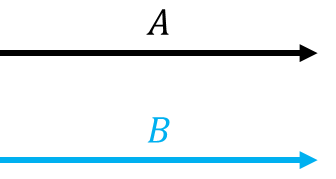
\includegraphics[width=0.9\linewidth]{./picture/1.png}
			\caption{Initial two route}
			\label{2opt 1}%文中引用该图片代号
		\end{minipage}
		\begin{minipage}{0.49\linewidth}
			\centering
			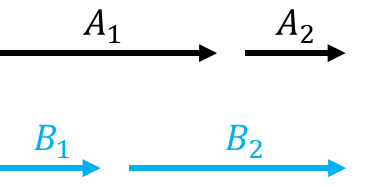
\includegraphics[width=0.9\linewidth]{./picture/2.png}
			\caption{Cut route}
			\label{2opt 2}%文中引用该图片代号
		\end{minipage}
		%\qquad
		%让图片换行,
		
		\begin{minipage}{0.49\linewidth}
			\centering
			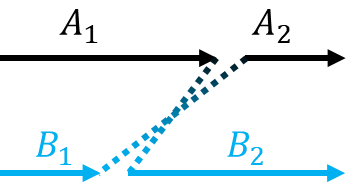
\includegraphics[width=0.9\linewidth]{./picture/3.png}
			\caption{Reproduced route 1}
			\label{2opt 3}%文中引用该图片代号
		\end{minipage}
		\begin{minipage}{0.49\linewidth}
			\centering
			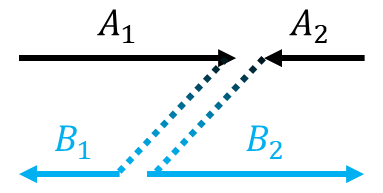
\includegraphics[width=0.9\linewidth]{./picture/4.png}
			\caption{Reproduced route 2}
			\label{2opt 4}%文中引用该图片代号
		\end{minipage}
	\end{figure}

	First randomly select two route as shown in Figure \ref{2opt 1}, written as $A$ and $B$. Then randomly choose a vertex on both edge, and cut edge into two parts as in Figure \ref{2opt 2}, where $A_1$ and $B_1$ contains start vertex, $A_2$ and $B_2$ contains end vertex. Then we have two ways to re-connect these four parts while maintain each reproduced edge have one start and one end: $A_1$ connects $B_2$ and $A_2$ connects $B_1$ in Figure \ref{2opt 3}, or $A_1$ connects reversed $B_1$ and reversed $A_2$ connects $B_2$ in Figure \ref{2opt 4}.

	\subsection{Selection}
	
	In this project, crossover is not considered. The new solution after mutation may be illegal, so a filter needs to be used to delete illegal solution, like exceed capacity limit. In the worst case, all of new solutions are illegal. So the process of generate initial population will repeat again. The next population will be select among mixed solutions from both process of initial population and from mutation. 
	

	\section{Experiment}\label{sec:experiment}
	
	After completing algorithm, some experiments needs to be done to ensure the optimization to algorithm works well, and to find out which parameter is better in practice. Here, each optimization is compared with random decision.
	
	\subsection{Setup}
	
	All experiments are implemented on following environment:
	
	\begin{table}[H]
		\begin{center}
			\caption{Experimental environment}
			\begin{tabular}{cp{6cm}}
				\toprule
				\textbf{Item} & \textbf{Configuration} \\
				\midrule
				Processor & AMD Ryzen 7 4800H with Radeon Graphics \\
				\specialrule{0em}{2pt}{2pt}
				RAM & 16.0GB\\
				\specialrule{0em}{2pt}{2pt}
				System & 64bit operation systen based on x64 processor \\
				\specialrule{0em}{2pt}{2pt}
				Operation system & Windows 10 Family Chinese Version, with version code 22H2 \\
				\specialrule{0em}{2pt}{2pt}
				OS inner version & 19045.2311 \\
				\specialrule{0em}{2pt}{2pt}
				IDE & Pycharm Professional 2022.3 \\
				\specialrule{0em}{2pt}{2pt}
				Python & 3.10 version \\
				\specialrule{0em}{2pt}{2pt}
				$numpy$ package & 1.21.5 version \\
				\bottomrule
			\end{tabular}
		\end{center}
	\end{table}
	
	\subsection{Test data}
	
	The graph for testing are as follows:
	
	\begin{table}[H]
		\begin{center}
			\caption{Testing graphs}
			\begin{tabular}{cccc}
				\toprule
				\textbf{Graph} & \textbf{Vertex number} & \textbf{Edge number} & \textbf{Demand edge number}\\
				\midrule
				egl-e1-A &$77$&$98$&$51 $\\
				\specialrule{0em}{2pt}{2pt}
				egl-s1-A &$ 140$&$190$&$75 $\\
				\specialrule{0em}{2pt}{2pt}
				gdb1 &$ 12$&$22$&$22 $\\
				\specialrule{0em}{2pt}{2pt}
				gdb10 &$ 12$&$25$&$25 $\\
				\specialrule{0em}{2pt}{2pt}
				val1A &$ 24$&$39$&$39 $\\
				\specialrule{0em}{2pt}{2pt}
				val4A &$ 41$&$69$&$69 $\\
				\specialrule{0em}{2pt}{2pt}
				val7A &$ 40$&$66$&$66 $\\
				\bottomrule
			\end{tabular}
		\end{center}
	\end{table}
	
	\subsection{Results}
	
	In experiments, flip, single insertion, double insertion, swap, 2-opt are run separately and compared with random selection on each decision in PS. Each competition for each mutation way is run for 100 times, 100 iteration of GA is run in each time. The number of winning and the improve percentage of average cost for each mutation way are shown in Table \ref{result}.
	
	All mutation way can reach global optimal cost for graph val1A, val4A, and val7A. If reach optimal cost, limit of mutation can't be observed. So all experiments are run on a relatively large graph: egl-e1-A.
	
	In experiments, the parameter of GA doesn't change for each competition. The parameter used is the final version of adjust. The method of adjust will be explained in 
	
	\begin{table}[H]
		\begin{center}
			\caption{Result of mutations $vs$ random}\label{result}
			\begin{tabular}{cccc}
				\toprule
				\textbf{Mutation} & \textbf{\makecell{Mutation\\win}} & \textbf{\makecell{Random\\win}} &  \textbf{\makecell{Cost\\improve}} \\
				\midrule
				Flip &$99$&$1$&$5.256\%$\\
				\specialrule{0em}{2pt}{2pt}
				\makecell{Single\\insertion} &$ 100$&$0$&$13.773\%$\\
				\specialrule{0em}{2pt}{2pt}
				\makecell{Double\\insertion} &$ 100$&$0$&$16.481\%$\\
				\specialrule{0em}{2pt}{2pt}
				\makecell{Swap} & $ 99$&$1$&$19.326\%$ \\
				\specialrule{0em}{2pt}{2pt}
				\makecell{2-opt}&$ 100$&$0$&$14.433\%$ \\
				\bottomrule
			\end{tabular}
		\end{center}
	\end{table}

	It can be seen that all of mutations can reach better solution than random chosen algorithm. Although random algorithm do win a few times, but consider the large number of experiments, it can be concluded that mutation is better than random under considerable error rate.
	
	\subsection{Adjust parameter}\label{adjust}
	
	There are some parameters in GA:
	
	\begin{itemize}
		\item Size of population
		\item One single solution is selected from how many solutions in process of initial population.
		\item How many solutions from process of initial population accounts in each generation of population
		\item How many solutions from mutation in each generation of population.
		\item How much time a single mutation way perform on a single route
		\item How many solutions are used for each mutation way.
	\end{itemize}

	All the parameters are adjusted by hand. That is, following sense to assign a initial value for each parameter, then run GA on large graph like egl-e1-A for multiple times. Observe the output of each time to determine whether this parameter is better than the previous one.

	
	
	% An example of a floating figure using the graphicx package.
	% Note that \label must occur AFTER (or within) \caption.
	% For figures, \caption should occur after the \includegraphics.
	% Note that IEEEtran v1.7 and later has special internal code that
	% is designed to preserve the operation of \label within \caption
	% even when the captionsoff option is in effect. However, because
	% of issues like this, it may be the safest practice to put all your
	% \label just after \caption rather than within \caption{}.
	%
	% Reminder: the "draftcls" or "draftclsnofoot", not "draft", class
	% option should be used if it is desired that the figures are to be
	% displayed while in draft mode.
	%
	%\begin{figure}[!t]
	%\centering
	%\includegraphics[width=2.5in]{myfigure}
	% where an .eps filename suffix will be assumed under latex, 
	% and a .pdf suffix will be assumed for pdflatex; or what has been declared
	% via \DeclareGraphicsExtensions.
	%\caption{Simulation results for the network.}
	%\label{fig_sim}
	%\end{figure}
	
	% Note that the IEEE typically puts floats only at the top, even when this
	% results in a large percentage of a column being occupied by floats.
	
	
	% An example of a double column floating figure using two subfigures.
	% (The subfig.sty package must be loaded for this to work.)
	% The subfigure \label commands are set within each subfloat command,
	% and the \label for the overall figure must come after \caption.
	% \hfil is used as a separator to get equal spacing.
	% Watch out that the combined width of all the subfigures on a 
	% line do not exceed the text width or a line break will occur.
	%
	%\begin{figure*}[!t]
	%\centering
	%\subfloat[Case I]{\includegraphics[width=2.5in]{box}%
		%\label{fig_first_case}}
	%\hfil
	%\subfloat[Case II]{\includegraphics[width=2.5in]{box}%
		%\label{fig_second_case}}
	%\caption{Simulation results for the network.}
	%\label{fig_sim}
	%\end{figure*}
	%
	% Note that often IEEE papers with subfigures do not employ subfigure
	% captions (using the optional argument to \subfloat[]), but instead will
	% reference/describe all of them (a), (b), etc., within the main caption.
	% Be aware that for subfig.sty to generate the (a), (b), etc., subfigure
	% labels, the optional argument to \subfloat must be present. If a
	% subcaption is not desired, just leave its contents blank,
	% e.g., \subfloat[].
	
	
	% An example of a floating table. Note that, for IEEE style tables, the
	% \caption command should come BEFORE the table and, given that table
	% captions serve much like titles, are usually capitalized except for words
	% such as a, an, and, as, at, but, by, for, in, nor, of, on, or, the, to
	% and up, which are usually not capitalized unless they are the first or
	% last word of the caption. Table text will default to \footnotesize as
	% the IEEE normally uses this smaller font for tables.
	% The \label must come after \caption as always.
	%
	%\begin{table}[!t]
	%% increase table row spacing, adjust to taste
	%\renewcommand{\arraystretch}{1.3}
	% if using array.sty, it might be a good idea to tweak the value of
	% \extrarowheight as needed to properly center the text within the cells
	%\caption{An Example of a Table}
	%\label{table_example}
	%\centering
	%% Some packages, such as MDW tools, offer better commands for making tables
	%% than the plain LaTeX2e tabular which is used here.
	%\begin{tabular}{|c||c|}
	%\hline
	%One & Two\\
	%\hline
	%Three & Four\\
	%\hline
	%\end{tabular}
	%\end{table}
	
	
	% Note that the IEEE does not put floats in the very first column
	% - or typically anywhere on the first page for that matter. Also,
	% in-text middle ("here") positioning is typically not used, but it
	% is allowed and encouraged for Computer Society conferences (but
	% not Computer Society journals). Most IEEE journals/conferences use
	% top floats exclusively. 
	% Note that, LaTeX2e, unlike IEEE journals/conferences, places
	% footnotes above bottom floats. This can be corrected via the
	% \fnbelowfloat command of the stfloats package.
	
	
	\section{Failed Attempts}
	
	In process of project, more methods are done to optimize algorithm. Due to various reasons, part of them failed.
	
	\subsection{Multiple insertion}
	
	This idea is inspired by ``double insertion''. Choose two different vertices in one randomly chosen route, cut off edges between these vertices, and insert into randomly chosen position among all routes.  
	
	In theory, multiple insertion is an extension of double insertion and single insertion, so its most optimal cost is better than single insertion and double insertion. However, after programming and test, it turns out that, possibility of better solution is too small that can be ignored.
	
	The problem is that, multiple insertion is ``too wide''. After some math calculation, even if only do multiple insertion one time at route, the mathematical expectation of changed edges is half of the whole route. That means, in more than 70\% percent of cases, the too long cut-down will make route it from and route it insert into illegal, just a waste of time.
	
	If time is infinite for each graph, then multiple insertion theoretically will get better answer than single insertion and double insertion. But because time limitation of this project, multiple insertion is not suitable.
	
	\subsection{PS-PT}
	
	A paper\cite{inproceedings} in 2022 October introduce a method combining Path Scanning and Partial Tour Building called ``PS-PT''.
	
	In summary, this method will preprocess whole graph, combine some edges with tiny demand into a large edge. And use this large edge to replace its component edges in original graph, so that these component edges are force to be traversed at same time during PS on edited graph. In paper, this method can obtain most optimal answer in 20\% to even 40\% cases.
	
	However, after two days of attempts and test, it is found that PS-PT can't be used. This project require to calculate cost on routes. And the cost is base on original graph, so graph itself can't be manipulated to keep demand function and cost function correct. If do Dijkstra or Floyd on original graph and calculate demand in edited graph, then all path passing edited edges will correct demand but incorrect cost. So this method isn't used in project.
	
	\section{Conclusion}
	Path Scanning based on six judging rules generate initial population in this project, each iteration mutate old population and select best solutions on new generation and mutated results in five ways. All mutations are proven to be better than random.
	
	
	
	
	% if have a single appendix:
	%\appendix[Proof of the Zonklar Equations]
	% or
	%\appendix  % for no appendix heading
	% do not use \section anymore after \appendix, only \section*
	% is possibly needed
	
	% use appendices with more than one appendix
	% then use \section to start each appendix
	% you must declare a \section before using any
	% \subsection or using \label (\appendices by itself
	% starts a section numbered zero.)
	%
	

	
	
	% Can use something like this to put references on a page
	% by themselves when using endfloat and the captionsoff option.
	\ifCLASSOPTIONcaptionsoff
	\newpage
	\fi
	
	
	
	% trigger a \newpage just before the given reference
	% number - used to balance the columns on the last page
	% adjust value as needed - may need to be readjusted if
	% the document is modified later
	%\IEEEtriggeratref{8}
	% The "triggered" command can be changed if desired:
	%\IEEEtriggercmd{\enlargethispage{-5in}}
	
	% references section
	
	% can use a bibliography generated by BibTeX as a .bbl file
	% BibTeX documentation can be easily obtained at:
	% http://mirror.ctan.org/biblio/bibtex/contrib/doc/
	% The IEEEtran BibTeX style support page is at:
	% http://www.michaelshell.org/tex/ieeetran/bibtex/
	%\bibliographystyle{IEEEtran}
	% argument is your BibTeX string definitions and bibliography database(s)
	%\bibliography{IEEEabrv,../bib/paper}
	%
	% <OR> manually copy in the resultant .bbl file
	% set second argument of \begin to the number of references
	% (used to reserve space for the reference number labels box)
	\bibliographystyle{acm}
	\bibliography{cited}
	
	% biography section
	% 
	% If you have an EPS/PDF photo (graphicx package needed) extra braces are
	% needed around the contents of the optional argument to biography to prevent
	% the LaTeX parser from getting confused when it sees the complicated
	% \includegraphics command within an optional argument. (You could create
	% your own custom macro containing the \includegraphics command to make things
	% simpler here.)
	%\begin{IEEEbiography}[{\includegraphics[width=1in,height=1.25in,clip,keepaspectratio]{mshell}}]{Michael Shell}
	% or if you just want to reserve a space for a photo:
	
	
	% insert where needed to balance the two columns on the last page with
	% biographies
	%\newpage

	
	% You can push biographies down or up by placing
	% a \vfill before or after them. The appropriate
	% use of \vfill depends on what kind of text is
	% on the last page and whether or not the columns
	% are being equalized.
	
	%\vfill
	
	% Can be used to pull up biographies so that the bottom of the last one
	% is flush with the other column.
	%\enlargethispage{-5in}
	
	
	
	% that's all folks
\end{document}


